\chapter[Modelagem de \textit{software}]{Modelagem de \textit{software}}

Este capítulo reúne os diagramas que representam os aspectos funcionais e estruturais do FlashFood: casos de uso, classes e modelo físico do banco de dados.

\section{Diagrama de casos de uso}

Para sintetizar as funcionalidades previstas e os perfis que interagem com o sistema, a Figura~\ref{fig:casos-de-uso} apresenta o diagrama de casos de uso do FlashFood.

\clearpage
\begin{figure}[p]
  \centering
  \caption{Diagrama de casos de uso do sistema FlashFood}
  \label{fig:casos-de-uso}
  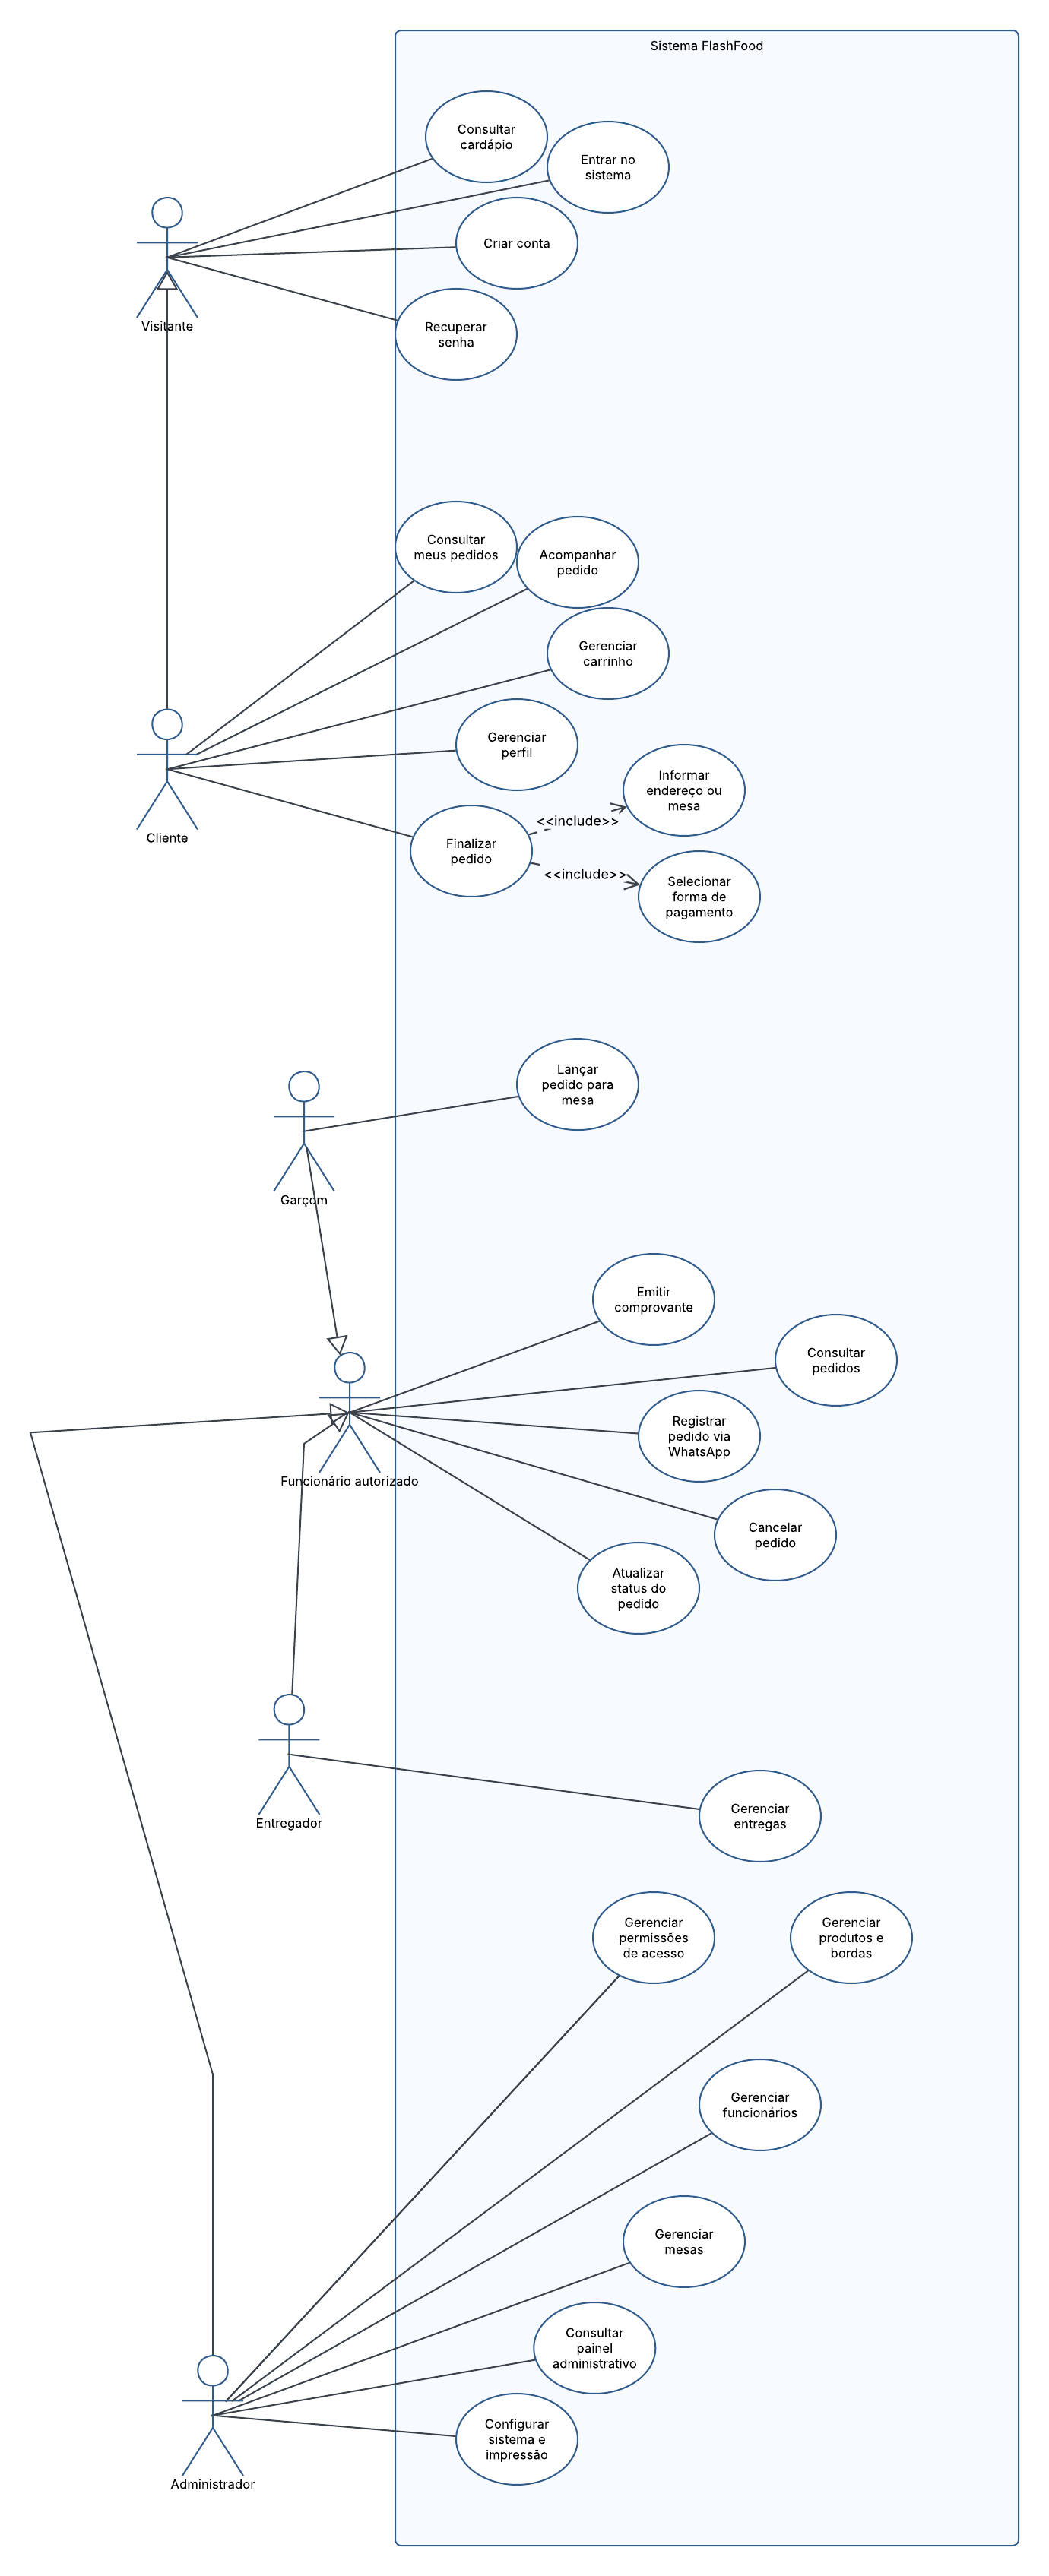
\includegraphics[height=0.88\textheight,keepaspectratio]{diagrama-caso-de-uso.png}
  \legend{Elaborado pelo autor (2026)}
\end{figure}
\clearpage

O visitante representa o usuário que ainda não está autenticado. Para esse perfil, o sistema disponibiliza a consulta ao cardápio, a criação de uma conta, o acesso ao sistema e a recuperação de senha. Após a autenticação, o cliente pode consultar e acompanhar pedidos, gerenciar o carrinho e o próprio perfil, além de finalizar uma compra.

Na finalização do pedido, o diagrama indica duas interações incluídas: informar o endereço ou a mesa e selecionar a forma de pagamento. A relação \texttt{<<include>>} representa etapas que fazem parte desse caso de uso, evidenciando as informações necessárias para registrar o pedido.

As atividades internas são distribuídas entre os demais perfis. O garçom pode lançar pedidos para mesas; o entregador pode gerenciar entregas; e o funcionário autorizado pode consultar pedidos, registrar pedidos recebidos pelo WhatsApp, cancelar pedidos, atualizar seus status e emitir comprovantes. O administrador, por sua vez, pode gerenciar produtos e bordas, funcionários, permissões e mesas, consultar o painel administrativo e configurar o sistema e a impressora.

As relações de generalização representadas no diagrama vinculam os papéis de garçom, entregador e administrador ao ator Funcionário autorizado. Essa organização reúne as operações comuns no perfil geral e mantém as funcionalidades específicas associadas a cada papel.

\section{Diagrama de classes}

Para facilitar a visualização das principais classes de domínio e de suas relações, a Figura~\ref{fig:modelo-classes} apresenta uma visão resumida do modelo de classes do sistema.

\clearpage
\begin{figure}[p]
  \centering
  \caption{Visão resumida do modelo de classes do sistema FlashFood}
  \label{fig:modelo-classes}
  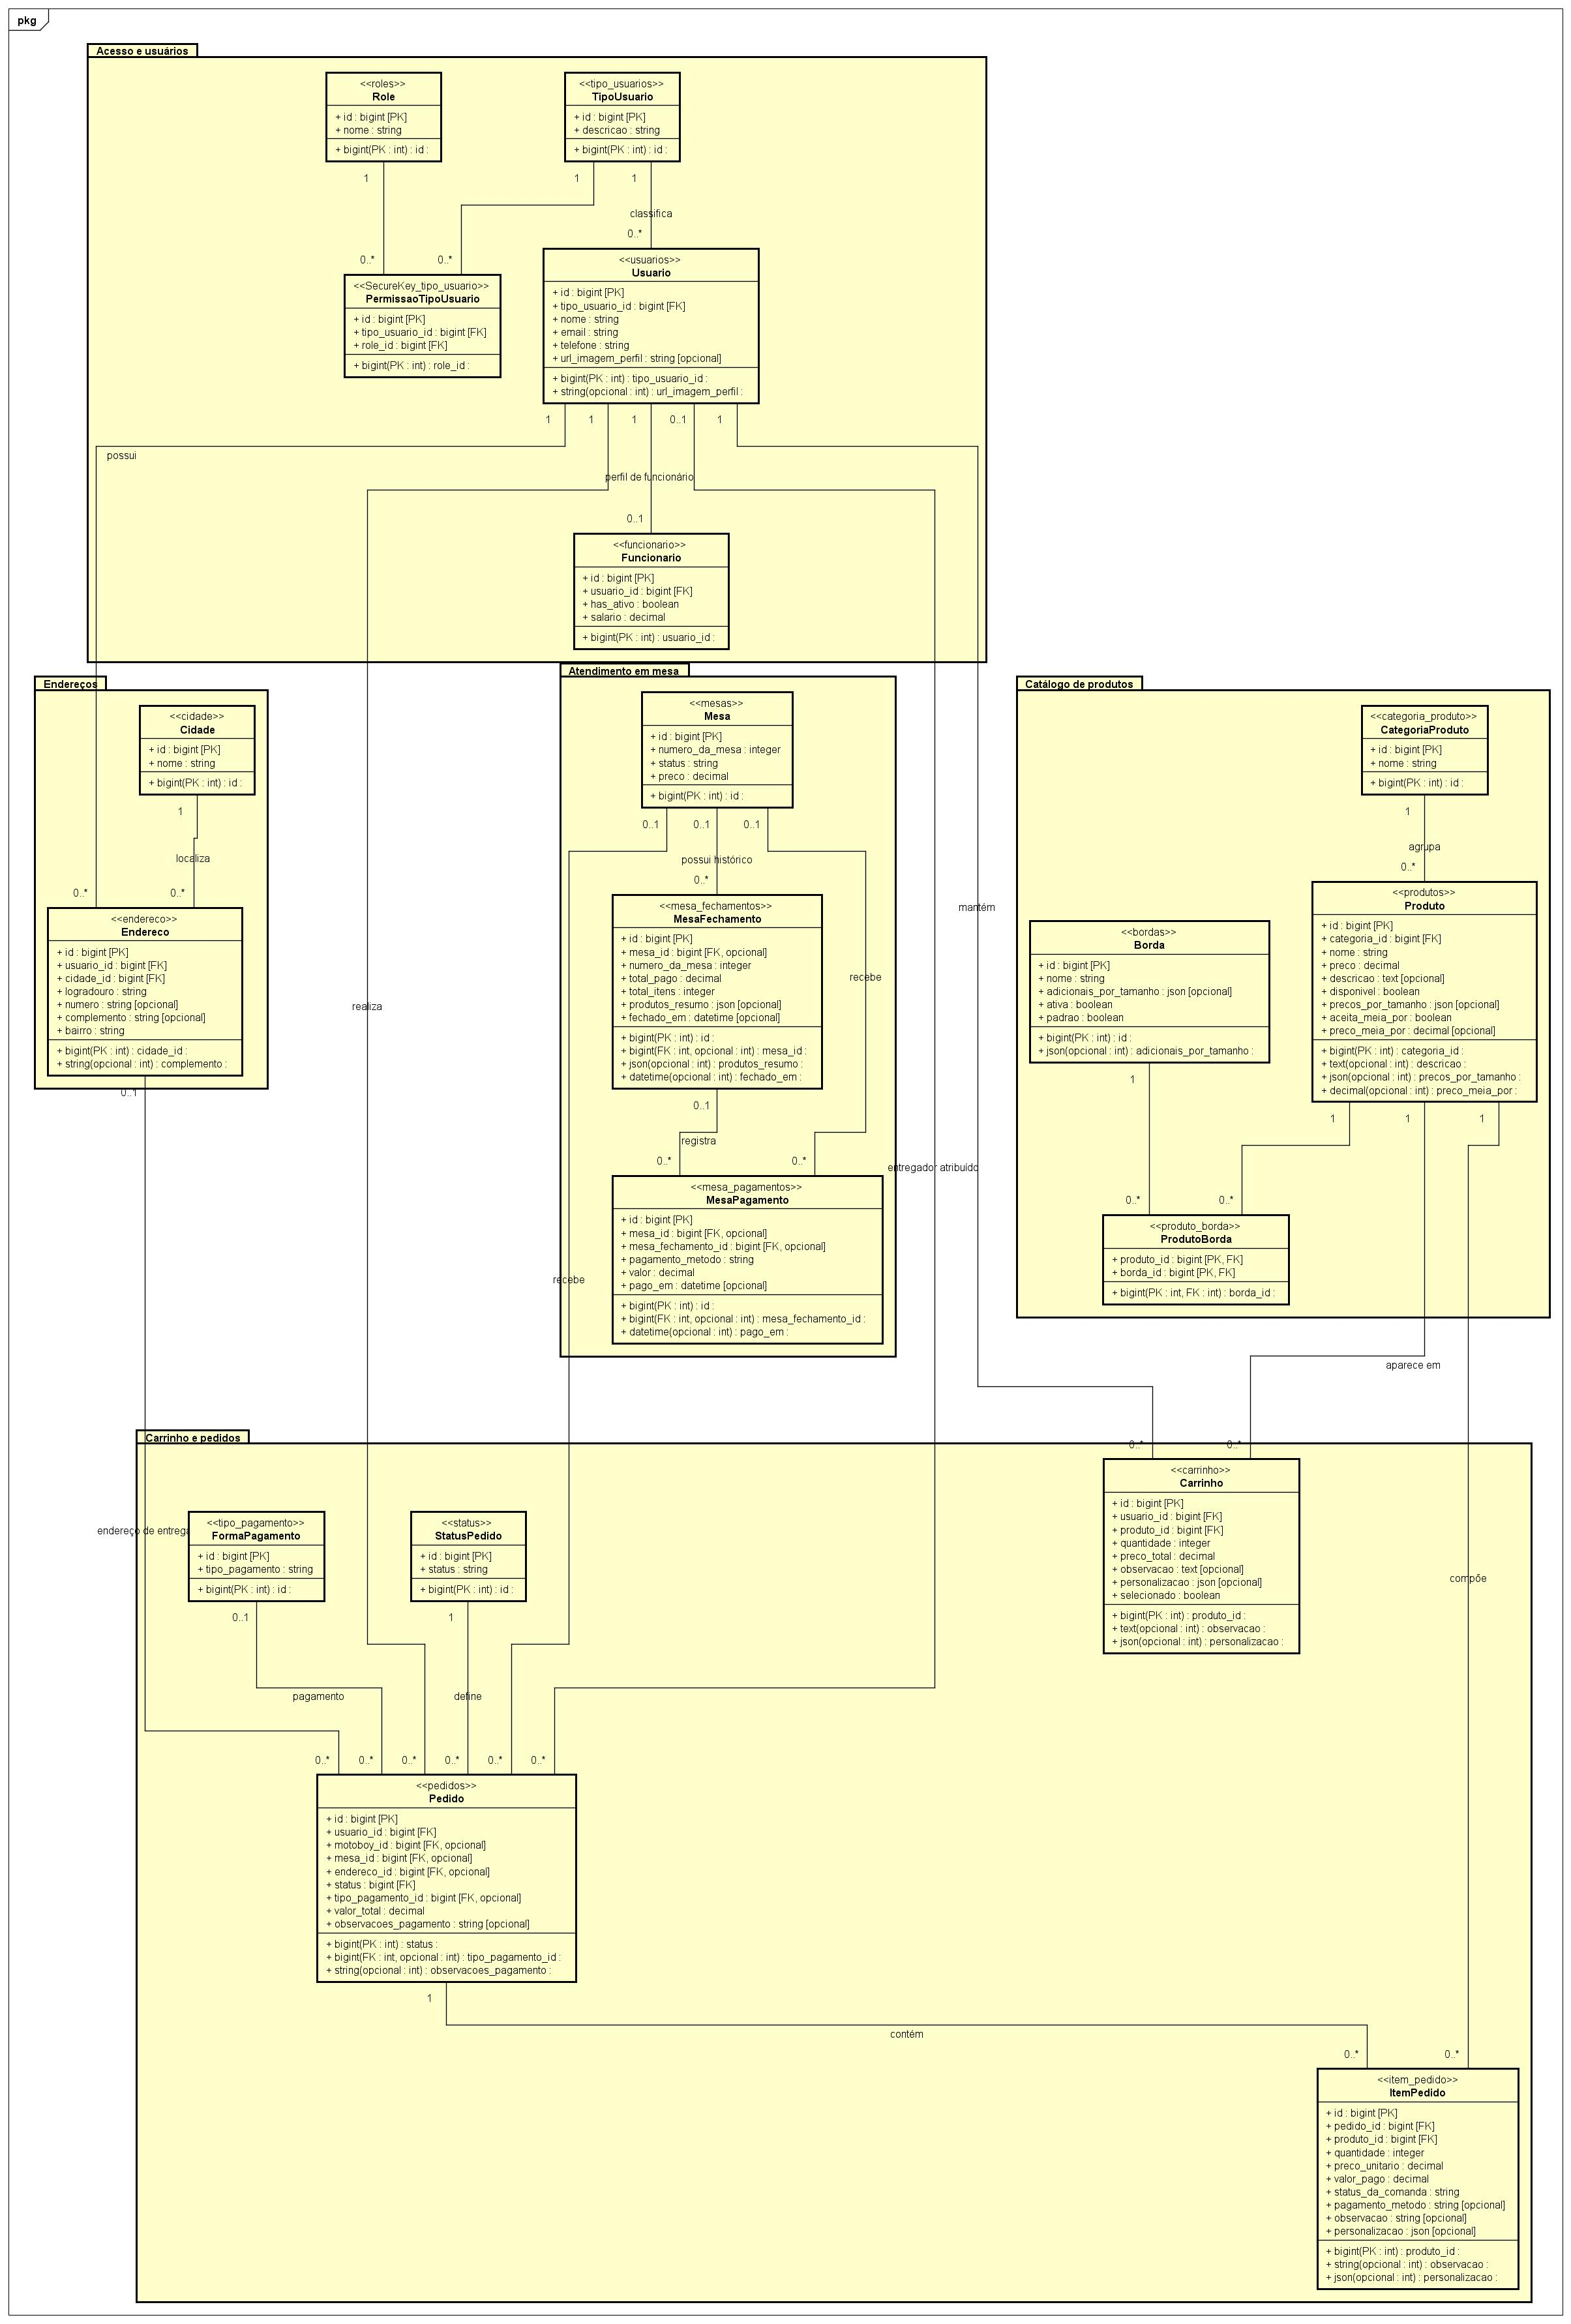
\includegraphics[height=0.88\textheight,keepaspectratio]{modelo-de-classes.jpg}
  \legend{Elaborado pelo autor (2026)}
\end{figure}
\clearpage

O modelo agrupa as classes por áreas do sistema, como acesso e usuários, endereços, atendimento em mesa, catálogo de produtos e carrinho e pedidos. As classes apresentam atributos e chaves, enquanto as associações e multiplicidades indicam como os registros se relacionam. A versão integral complementa essa visão com as classes de controle, serviços, repositórios e suas implementações, \textit{middleware}, mensagens e enumerações. Devido à quantidade de elementos, o diagrama completo pode ser acessado pelo endereço: \url{https://github.com/RIGUETE-PEDRO/FlashFood/blob/main/diagramaClasse.jpg}.

\section{Modelo f\'isico do banco de dados}

A Figura~\ref{fig:flashfood-fisico} apresenta a vis\~ao geral do banco de dados. Para facilitar a leitura das tabelas e de seus campos, as amplia\c{c}\~oes das diferentes regi\~oes est\~ao nas Figuras~\ref{fig:flashfood-detalhe-1} a~\ref{fig:flashfood-detalhe-4}.

\clearpage
\begin{landscape}
\begin{figure}[p]
  \centering
  \begin{minipage}{0.77\linewidth}
    \caption{Modelo f\'isico do banco de dados do sistema FlashFood (vis\~ao geral)}
    \label{fig:flashfood-fisico}
    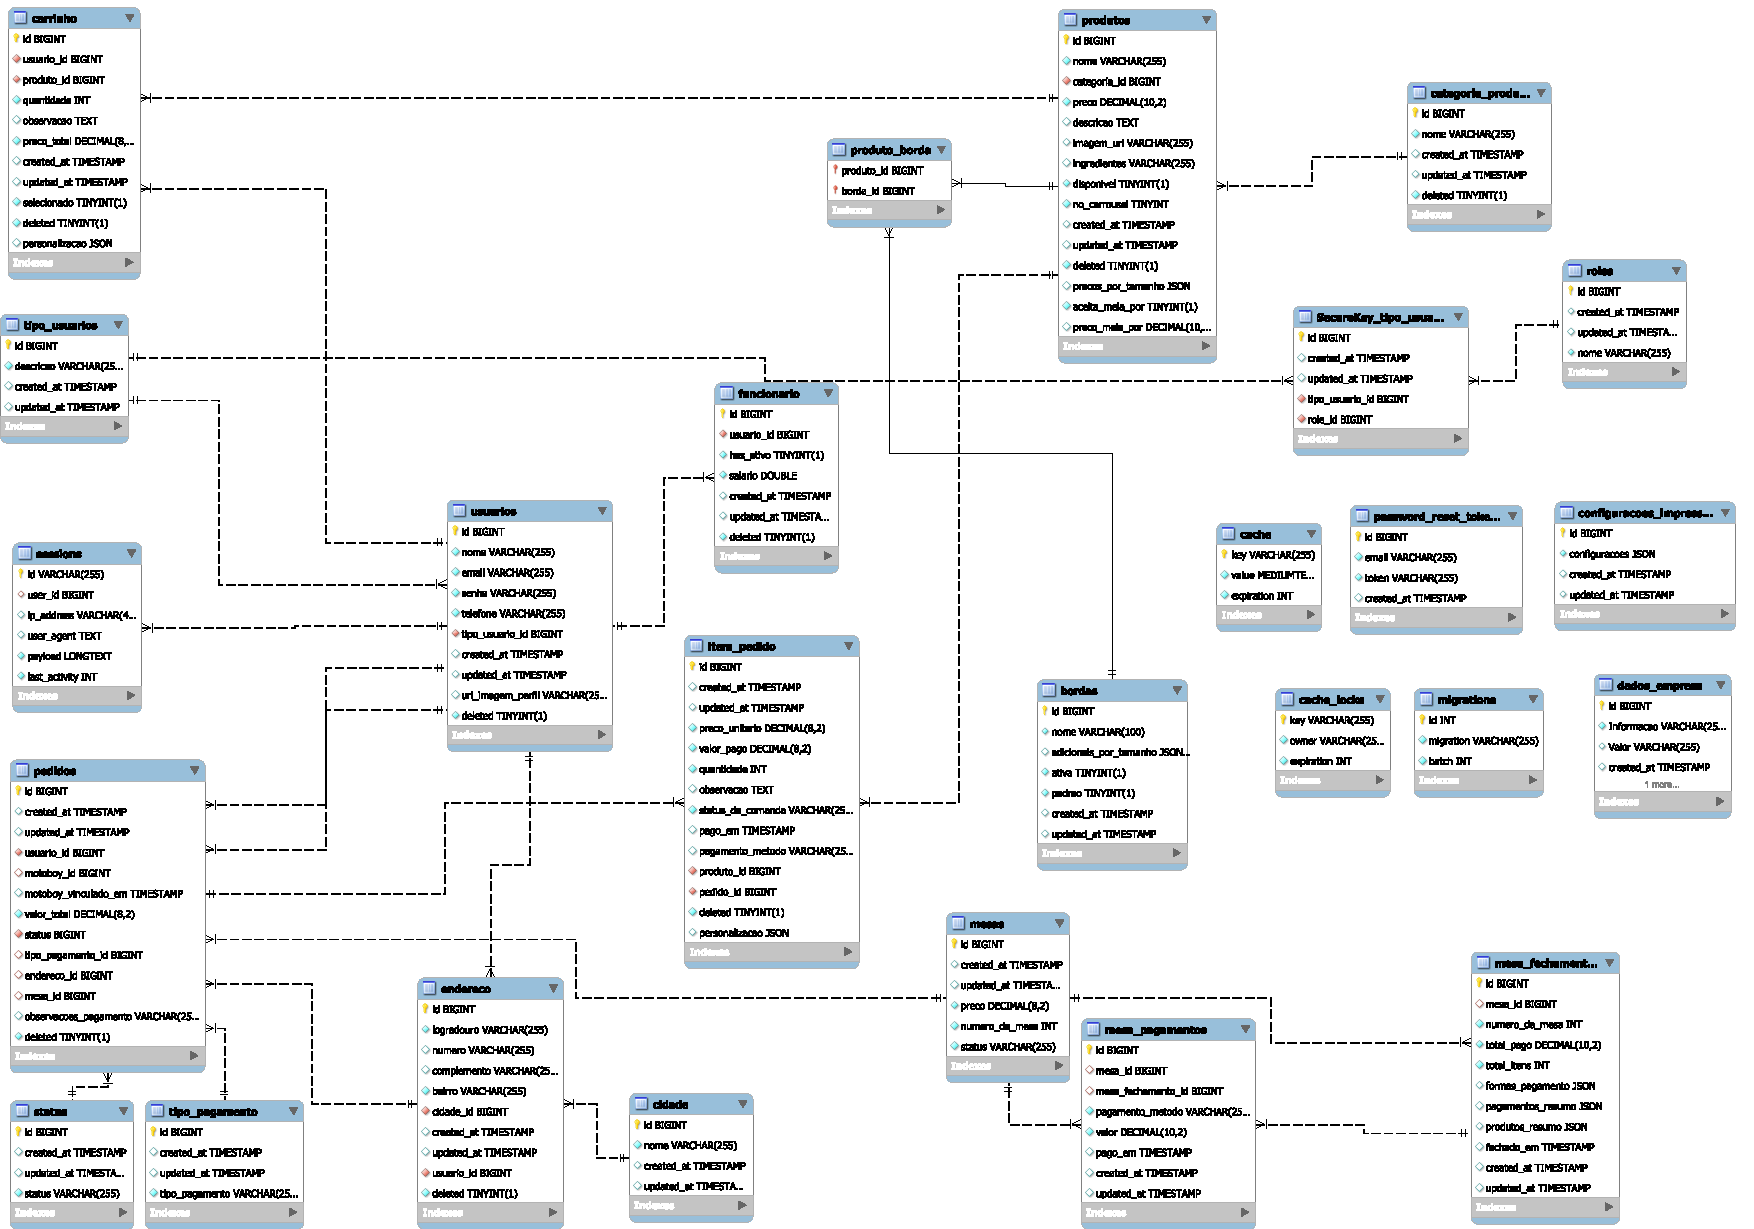
\includegraphics[width=\linewidth]{modelo-banco-organizado.pdf}
    \legend{ Elaborado pelo autor (2026)}
  \end{minipage}
\end{figure}
\end{landscape}
\clearpage

\begin{landscape}
\begin{figure}[p]
  \centering
  \begin{minipage}{0.71\linewidth}
    \caption{Detalhe do modelo f\'isico do banco de dados -- regi\~ao superior esquerda}
    \label{fig:flashfood-detalhe-1}
    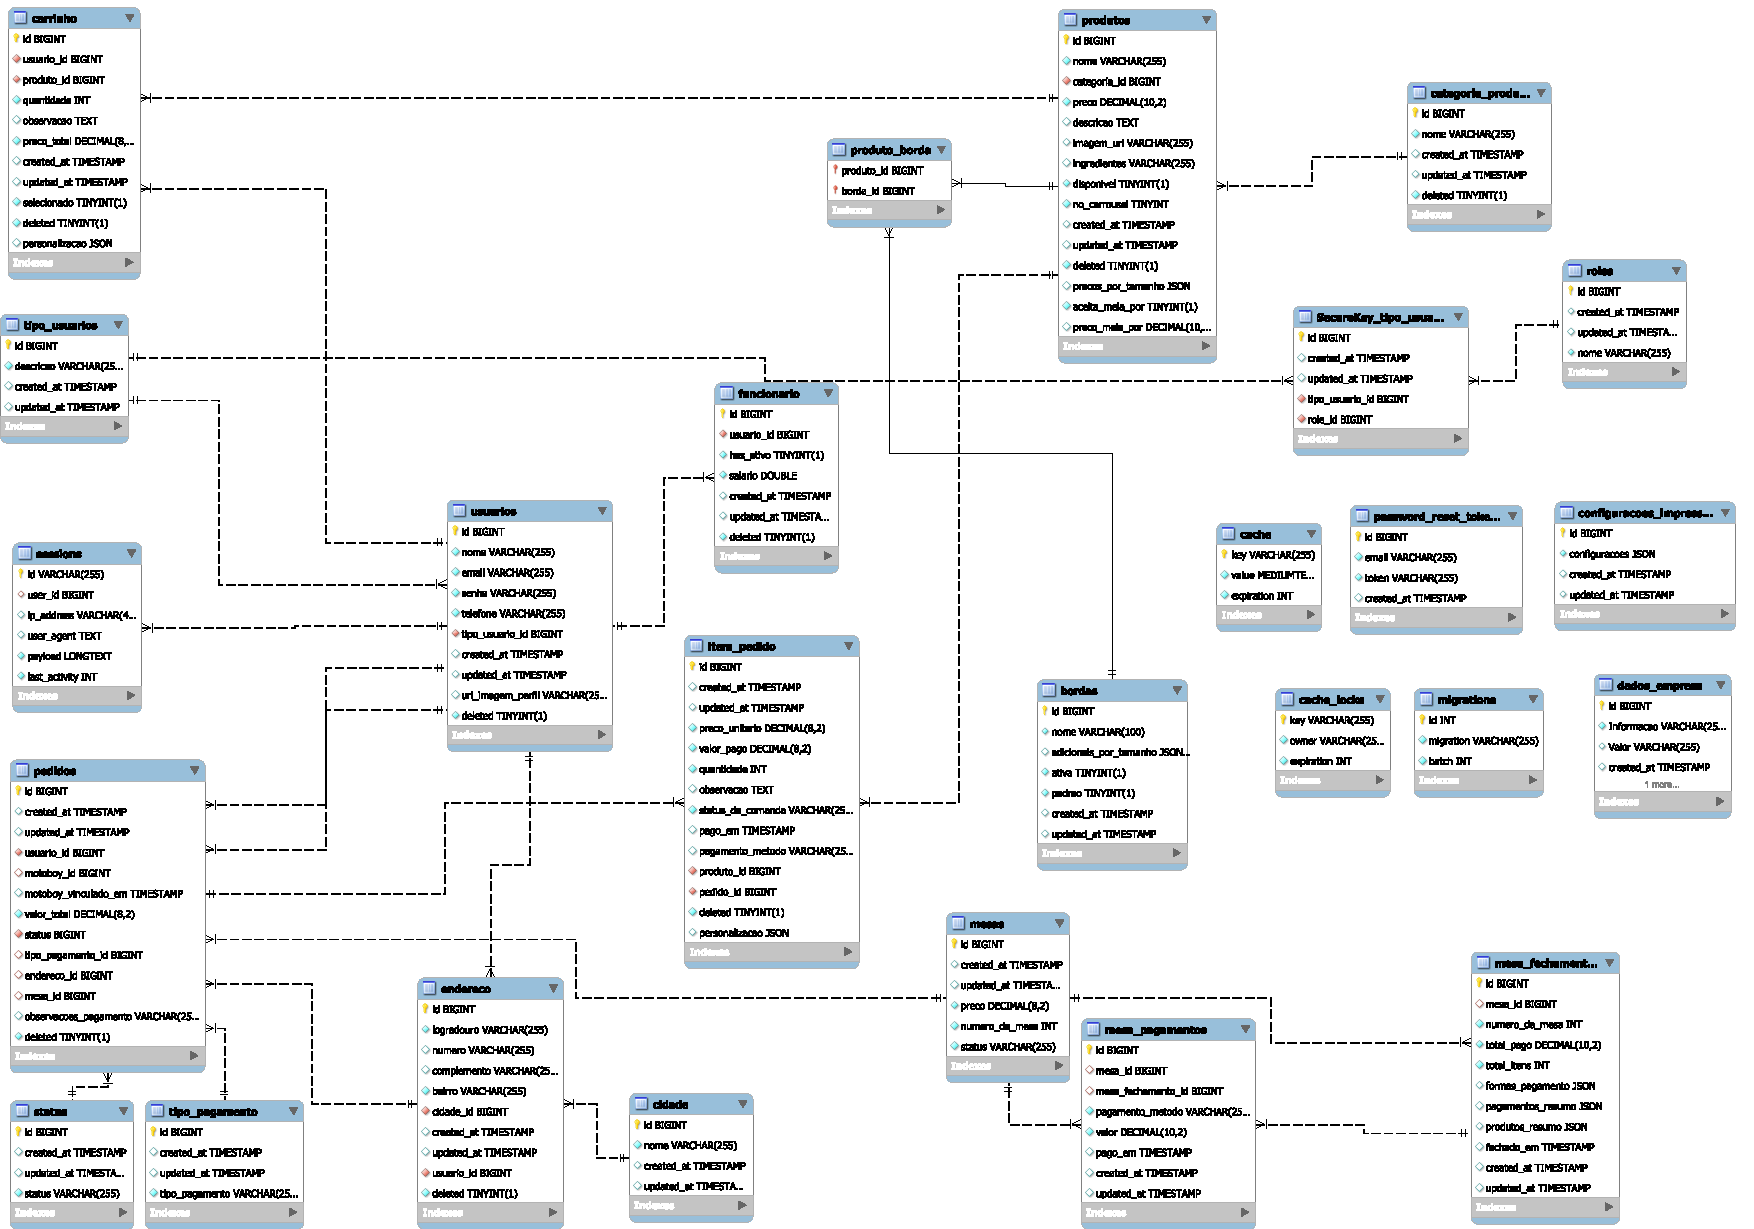
\includegraphics[width=\linewidth,trim=0pt 256pt 400pt 0pt,clip]{modelo-banco-organizado.pdf}
    \legend{ Elaborado pelo autor (2026)}
  \end{minipage}
\end{figure}
\end{landscape}
\clearpage

\begin{landscape}
\begin{figure}[p]
  \centering
  \begin{minipage}{0.79\linewidth}
    \caption{Detalhe do modelo f\'isico do banco de dados -- regi\~ao superior direita}
    \label{fig:flashfood-detalhe-2}
    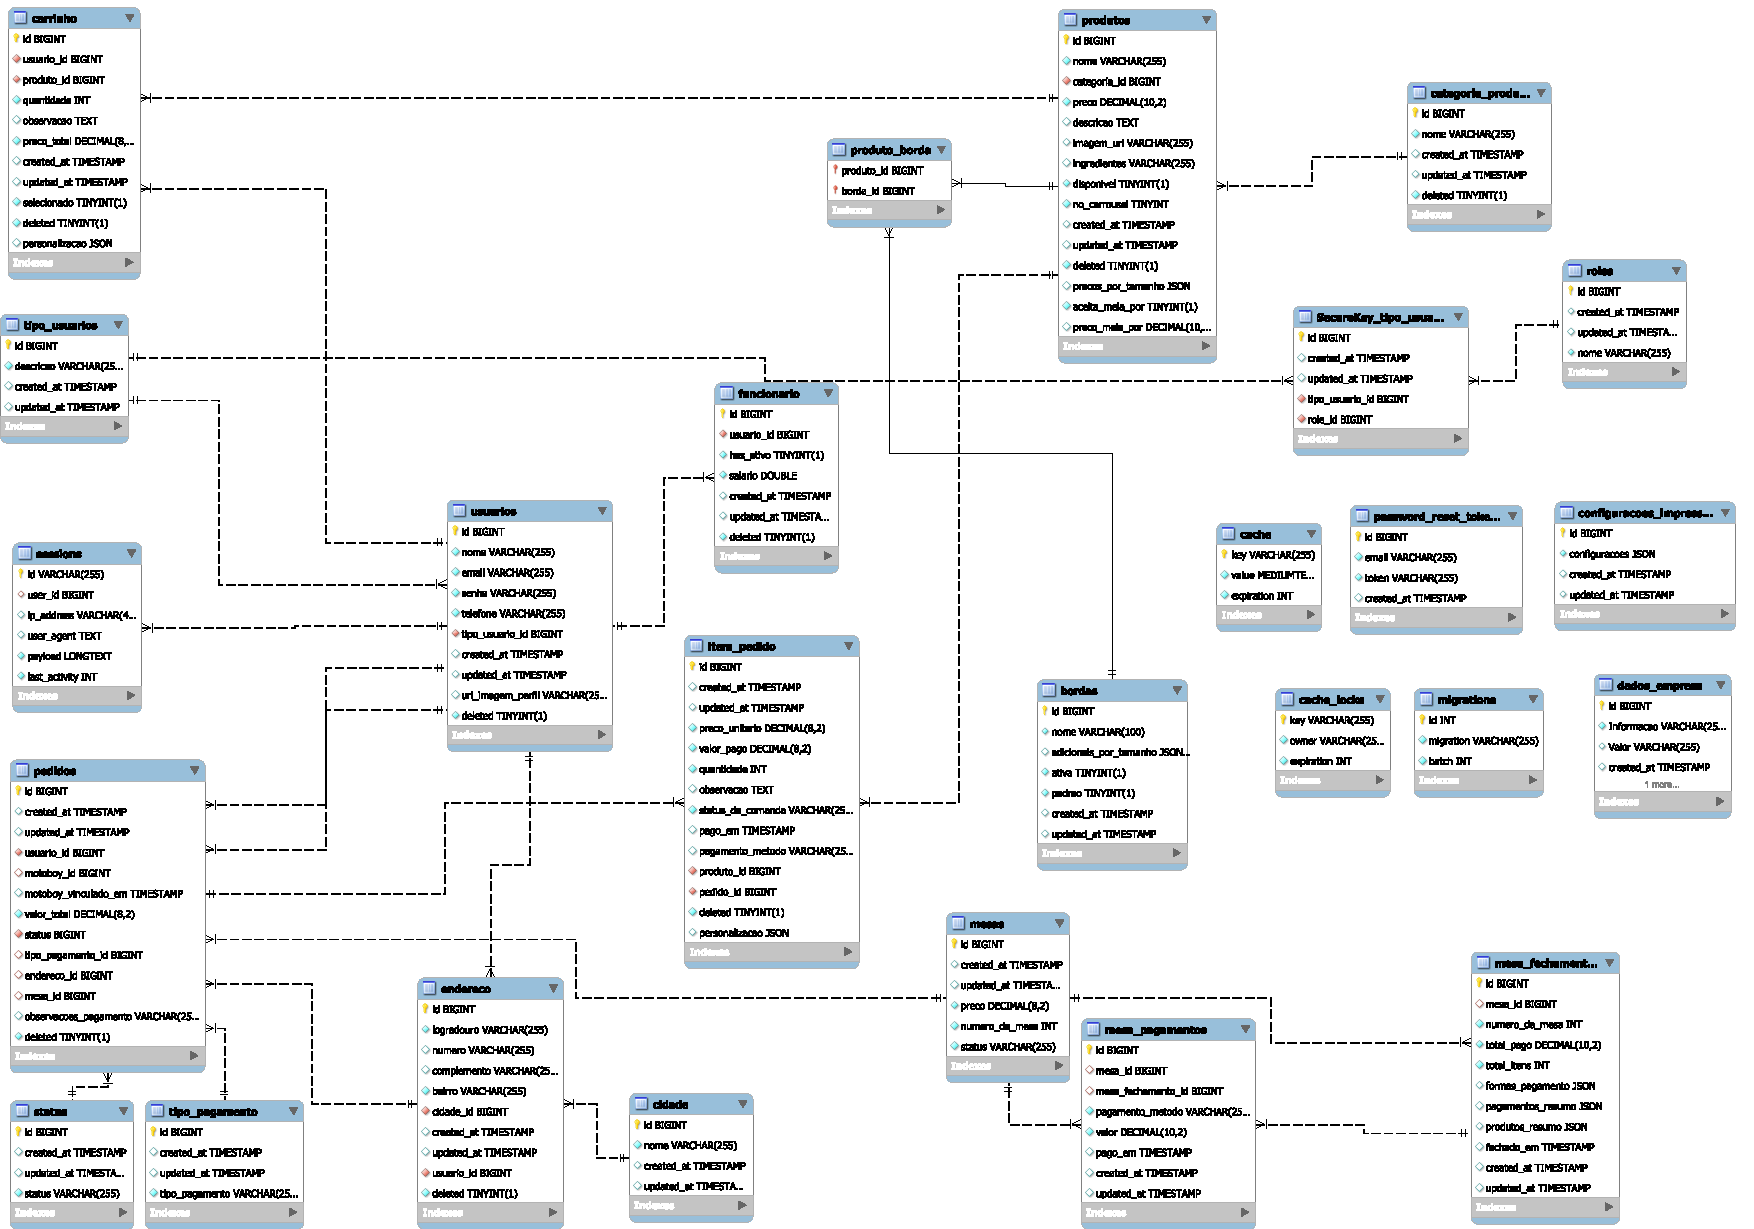
\includegraphics[width=\linewidth,trim=350pt 256pt 0pt 0pt,clip]{modelo-banco-organizado.pdf}
    \legend{ Elaborado pelo autor (2026)}
  \end{minipage}
\end{figure}
\end{landscape}
\clearpage

\begin{landscape}
\begin{figure}[p]
  \centering
  \begin{minipage}{0.68\linewidth}
    \caption{Detalhe do modelo f\'isico do banco de dados -- regi\~ao inferior esquerda}
    \label{fig:flashfood-detalhe-3}
    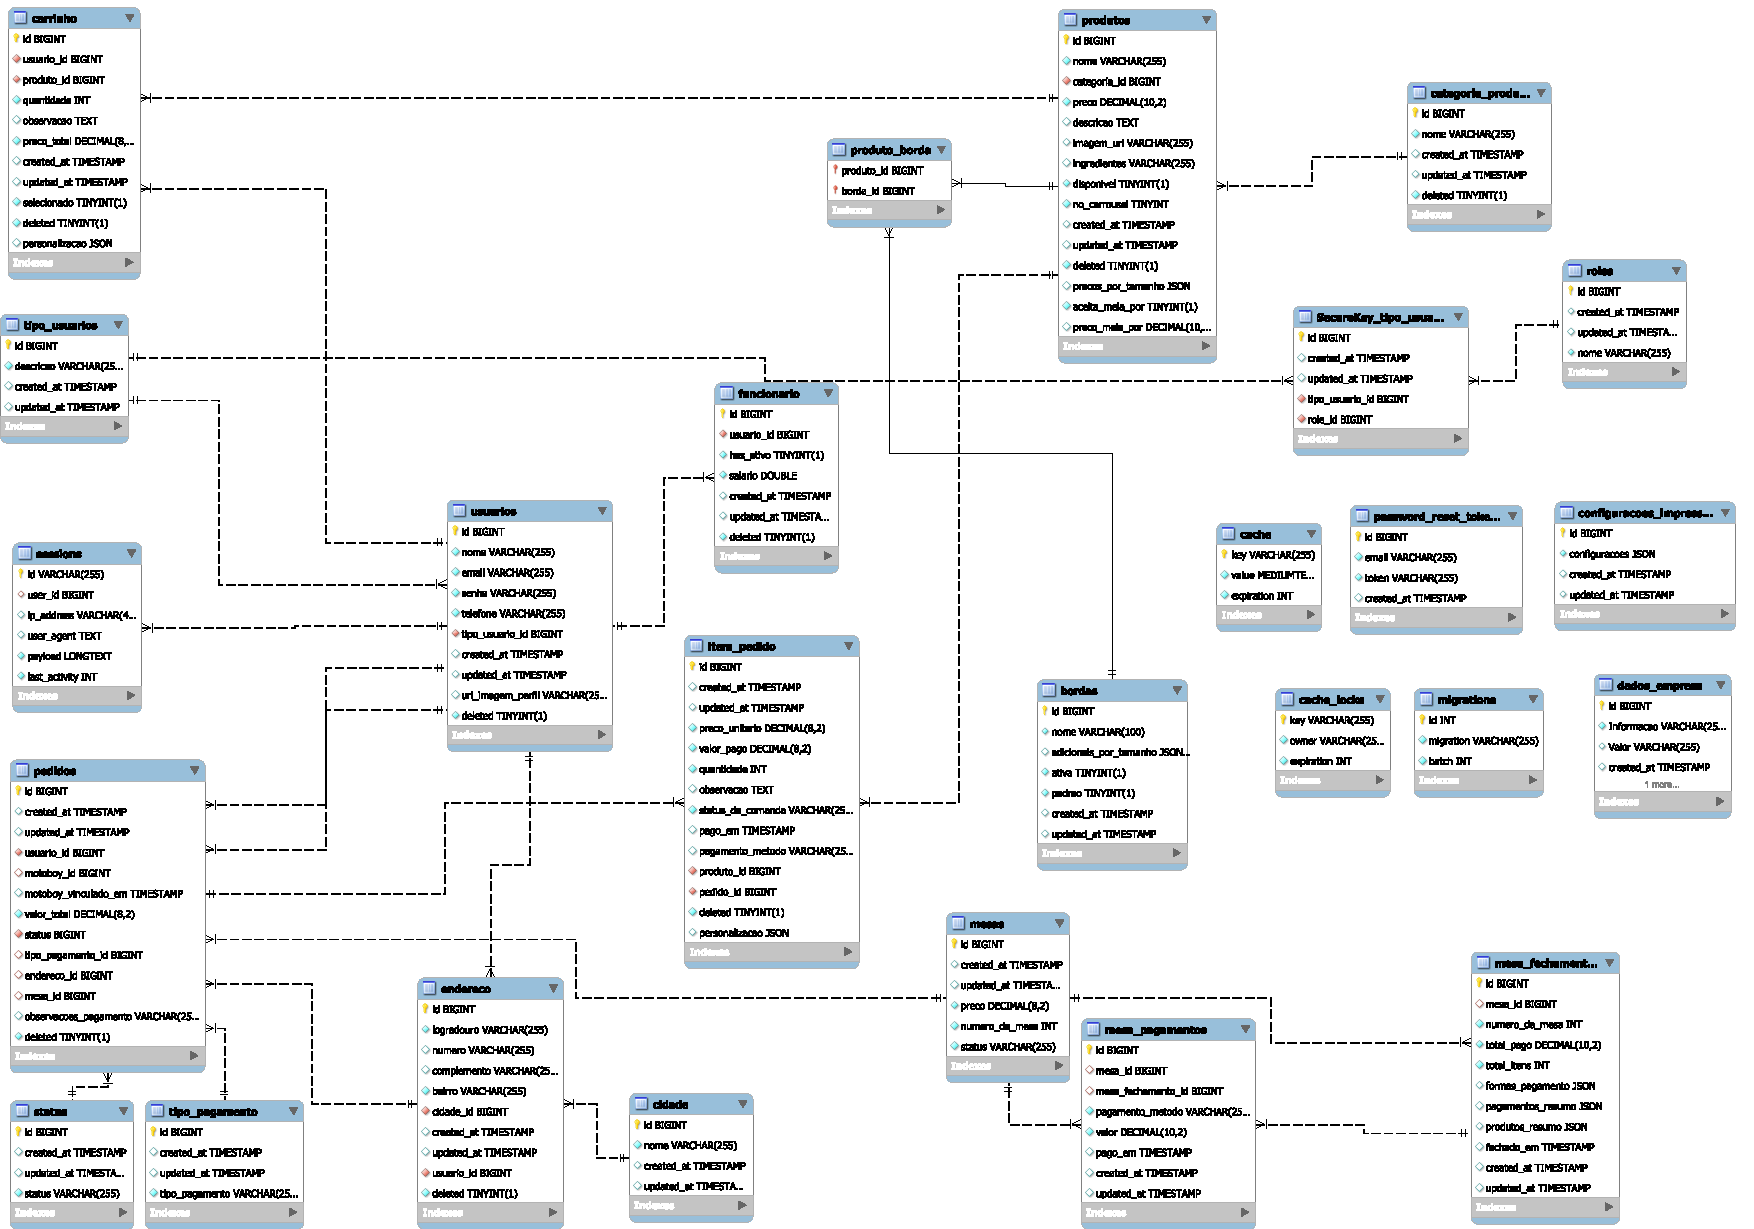
\includegraphics[width=\linewidth,trim=0pt 0pt 400pt 243pt,clip]{modelo-banco-organizado.pdf}
    \legend{ Elaborado pelo autor (2026)}
  \end{minipage}
\end{figure}
\end{landscape}
\clearpage

\begin{landscape}
\begin{figure}[p]
  \centering
  \begin{minipage}{0.76\linewidth}
    \caption{Detalhe do modelo f\'isico do banco de dados -- regi\~ao inferior direita}
    \label{fig:flashfood-detalhe-4}
    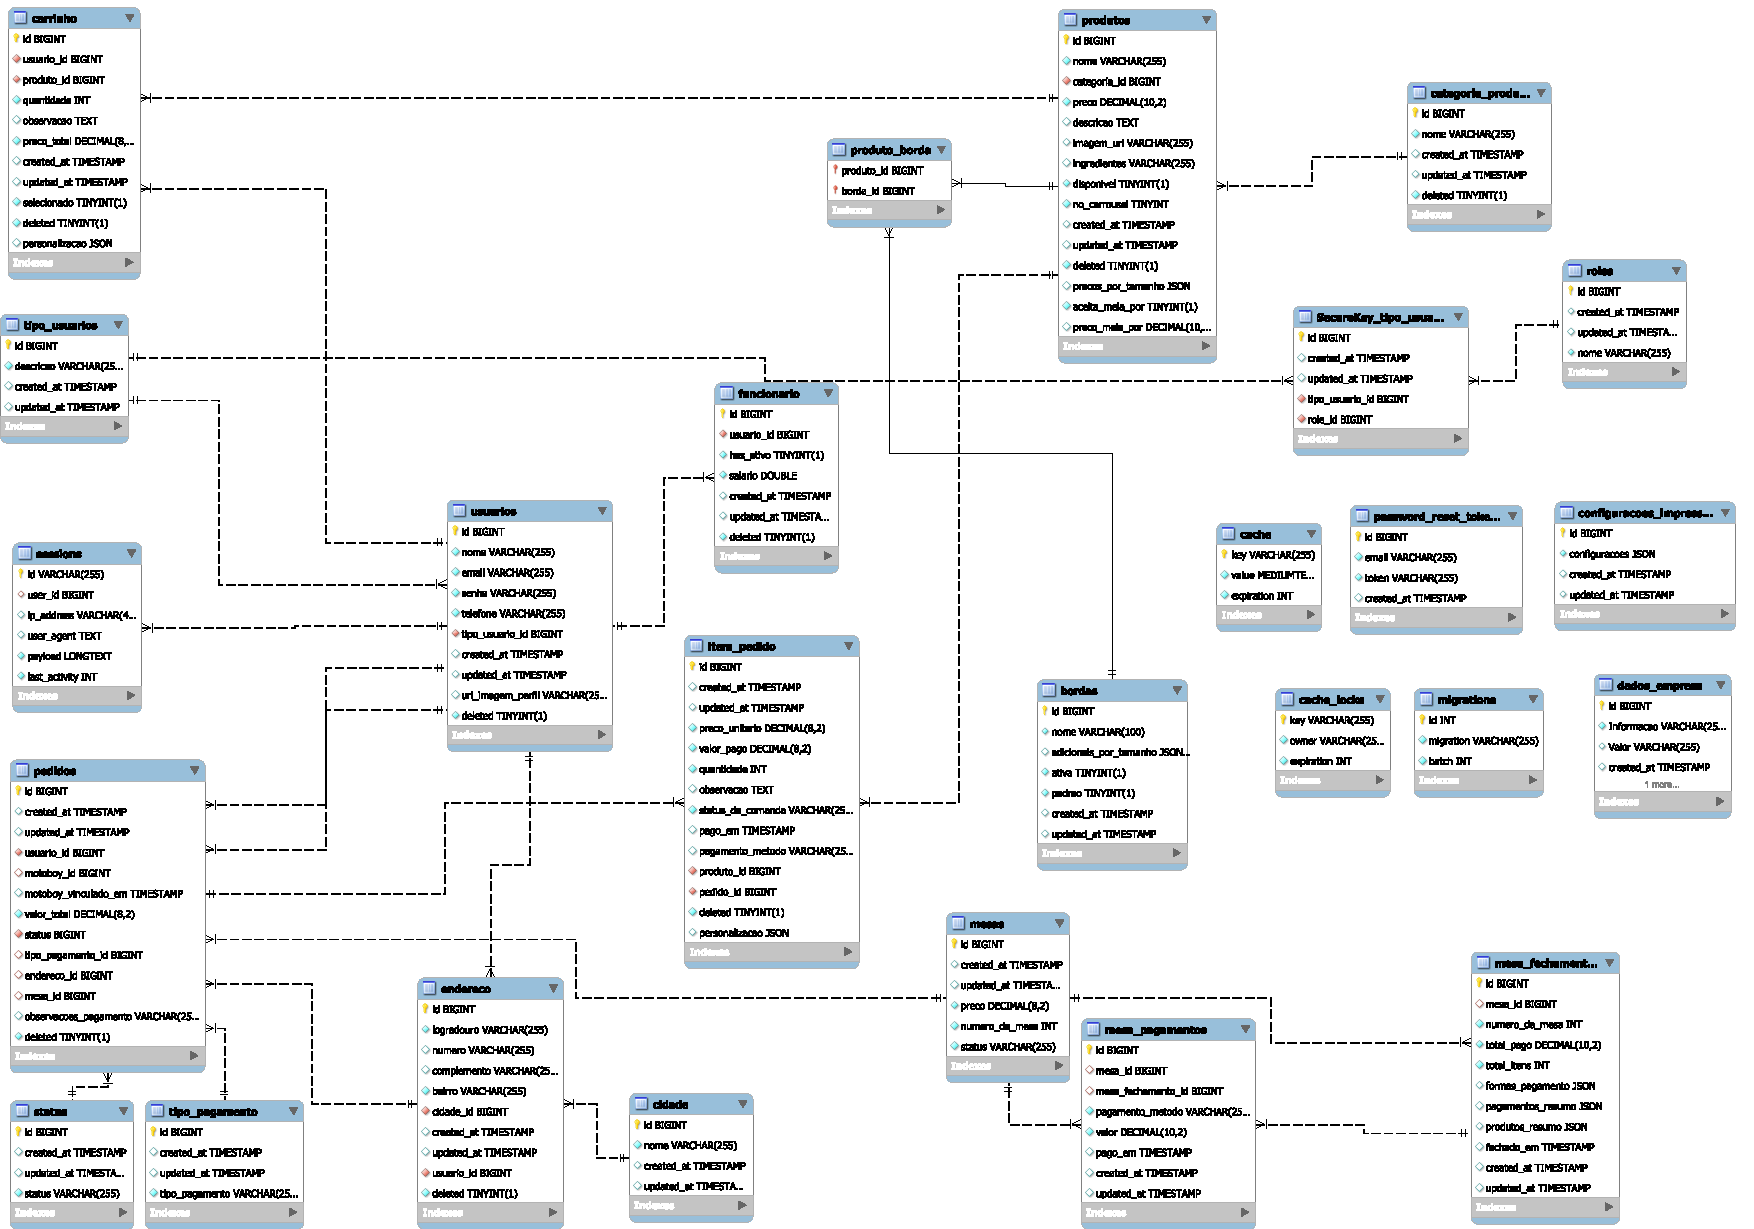
\includegraphics[width=\linewidth,trim=350pt 0pt 0pt 243pt,clip]{modelo-banco-organizado.pdf}
    \legend{ Elaborado pelo autor (2026)}
  \end{minipage}
\end{figure}
\end{landscape}
\clearpage
